\subsection{Gaussian Mixture}
\label{sec:ctm-gm}

The second clustering algorithm we tried was Gaussian Mixture \cite{dempster1977maximum}. Similar to the K-Means algorithm, it also groups unlabeled data points but with different criteria. As its name suggests, it assumes the points are randomly distributed following a Gaussian distribution. It iteratively tries to assign groups to maximize the likelihood of each data point belonging to their assigned groups. Likewise, we hypothesized that the closer a point (student solution) is to the centroid, in this case the central probability contour, the higher the probability of the student receiving a high score. In practice, we designated each student's score to be equal to the probability of them belonging to their assigned cluster, returned from the Gaussian Mixture algorithm.

\begin{figure}
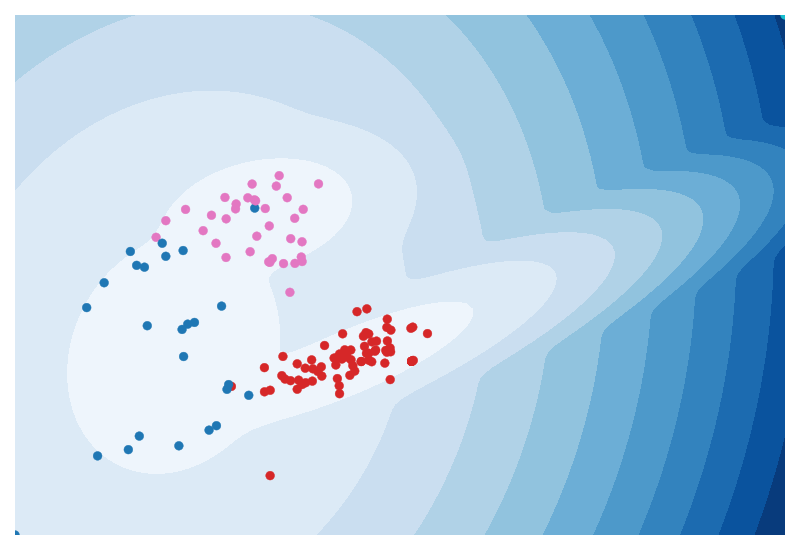
\includegraphics[width=\textwidth]{conversion-to-mark/marking_paster_nbio_ece459-a1-w2017_gm}
\caption[Gaussian Mixture Clustering]{This is a probability contour graph of our data points grouped by the Gaussian Mixture algorithm. Points closer to the center of the contours, i.e. lighter areas, have a higher probability of belonging to their corresponding group.}
\label{fig:ctm-gm}
\end{figure}
